\documentclass[aspectratio=169]{beamer}

% IEEE Style Theme Configuration
\usetheme{Madrid}
\usecolortheme{whale}

% Packages
\usepackage{graphicx}
\usepackage{amsmath}
\usepackage{booktabs}
\usepackage{bm}

% Title Information
\title[SOC Estimation via MO-ACO-EKF]{Ant-Colony-Optimized Extended Kalman Filter \\ for State of Charge Estimation of Li-Ion Batteries}
\author[Team]{%
    G. Jyothish (CB.AI.U4AID24114) \\
    J. S. Badri (CB.AI.U4AID24120) \\
    K. Chakradhar Reddy (CB.AI.U4AID24122) \\
    Sandeep S (CB.AI.U4AID24149) \\
    \vspace{0.3cm} \small Guide: [Insert Guide Name]%
}
\institute[Amrita Vishwa Vidyapeetham]{Department of Artificial Intelligence}
\date{\today}

\begin{document}

% SLIDE 1: Title
\begin{frame}
    \titlepage
\end{frame}

% SLIDE 2: Problem Statement & Objective
\begin{frame}{Problem Statement \& Objective}
    \textbf{The Problem:}
    \begin{itemize}
        \item State of Charge (SOC) acts as the "fuel gauge" for EVs but cannot be measured directly.
        \item Highly dynamic EV driving and extreme temperatures cause severe sensor noise and non-linear battery degradation.
        \item Traditional filters suffer from human-error in parameter guessing and mathematical instability (crashing) during long drives.
    \end{itemize}
    \vspace{0.5cm}
    \textbf{Project Objective:}
    \begin{itemize}
        \item To develop a highly accurate, temperature-adaptive SOC estimation system using a 3-State Extended Kalman Filter (EKF). 
        \item To ensure absolute stability and precision by optimizing the filter's noise covariance matrices using Multi-Objective Ant Colony Optimization (MO-ACO).
    \end{itemize}
\end{frame}

% SLIDE 3: Introduction
\begin{frame}{Introduction to SOC Estimation}
    \begin{block}{What is SOC?}
        SOC represents the remaining available energy in a battery, scaled from 0\% (empty) to 100\% (full). Accurate estimation prevents overcharging, extends lifespan, and eliminates EV range anxiety.
    \end{block}
    \vspace{0.3cm}
    \textbf{Measurement Challenges:}
    \begin{itemize}
        \item We can only measure Voltage ($V$), Current ($I$), and Temperature ($T$).
        \item Battery chemistry is highly non-linear. Rapid acceleration causes drastic voltage drops that do not immediately reflect true SOC.
        \item We must use a software "Digital Twin" to mathematically guess the internal state based on these external sensors.
    \end{itemize}
\end{frame}

% SLIDE 4: Motivation
\begin{frame}{Motivation}
    Why is an advanced approach necessary?
    \begin{itemize}
        \item \textbf{Preventing Catastrophic Failures:} Inaccurate SOC causes Battery Management Systems (BMS) to overcharge cells, leading to thermal runaway and fires.
        \item \textbf{The Temperature Problem:} Most existing algorithms fail during winter freezing or summer fast-charging. We are motivated to include Arrhenius Thermal Physics.
        \item \textbf{Mathematical Robustness:} Standard Kalman Filters often crash due to floating-point rounding errors on EV microcontrollers. We use a Joseph-Form update to guarantee the software never crashes.
    \end{itemize}
\end{frame}

% SLIDE 5: Literature Review
\begin{frame}{Literature Review}
    \begin{table}[]
        \centering
        \resizebox{\textwidth}{!}{%
        \begin{tabular}{@{}llll@{}}
        \toprule
        \textbf{Key Papers} & \textbf{Methodology} & \textbf{Core Results} & \textbf{Key Limitations} \\ \midrule
        Chen et al. (2019)  & OCV-SOC Mapping  & Perfect in resting state & Completely fails during active dynamic driving. \\
        Wang \& Li (2020)   & Standard EKF    & Tracks dynamic driving   & Matrices (Q, R) rely on human guesswork. \\
        Zhang et al. (2021) & Thermal 2-RC    & Good in cold weather     & Heavy math causes filter instability (crashes). \\
        Kumar et al. (2022) & PSO Optimization& AI-tuned parameters      & Ignored thermal physics; weak in varying climates. \\ \bottomrule
        \end{tabular}%
        }
    \end{table}
    \vspace{0.3cm}
    \textbf{Research Gap:} Existing methods lack a unified solution that combines AI-optimized parameters, thermal adaptability, and mathematical stability.
\end{frame}

% SLIDE 7: Proposed Methodology (System Architecture)
\begin{frame}{Proposed Methodology: System Architecture}
    Our proposed architecture follows a structured Model-Based Design (MBD):
    \begin{enumerate}
        \item \textbf{EV Driving Conditions:} Synthetic generation of dynamic drive cycles (UDDS, Highway, Pulse).
        \item \textbf{2-RC Thermal Plant:} A mathematical digital twin simulating exact electrochemical responses.
        \item \textbf{Sensor Measurement:} Addition of realistic hardware Gaussian noise ($\pm$8mV ADC, $\pm$0.5K Temp).
        \item \textbf{MO-ACO Optimizer:} Offline AI algorithm to determine optimal $Q^*$ and $R^*$ matrices.
        \item \textbf{ACO-EKF Controller:} The 3-State Brain utilizing Joseph-Form updates to predict True SOC.
    \end{enumerate}
\end{frame}

% SLIDE 8: Battery Modeling (2-RC Thermal)
\begin{frame}{Battery Modeling: 2-RC Thermal-Adaptive Model}
    We modeled the battery using a 2-RC Equivalent Circuit:
    \begin{itemize}
        \item \textbf{Activation Polarization ($R_1, C_1$):} Captures fast surface-level chemical reactions.
        \item \textbf{Concentration Polarization ($R_2, C_2$):} Captures slow, deep-liquid ion movement.
    \end{itemize}
    \vspace{0.3cm}
    \textbf{Thermal Coupling (Arrhenius Equation):}
    \begin{equation}
        t_{factor} = \exp\left(\frac{E_a}{R_{gas}} \left(\frac{1}{T_{meas}} - \frac{1}{T_{ref}}\right)\right)
    \end{equation}
    This dynamically alters the internal resistance based on real-time temperature, mimicking freezing and overheating conditions perfectly.
\end{frame}

% SLIDE 9: The Extended Kalman Filter (Joseph-Form)
\begin{frame}{The BMS Brain: Extended Kalman Filter}
    The EKF filters out real-world noise through a strict mathematical loop:
    \begin{enumerate}
        \item \textbf{Prediction:} The model guesses current SOC and Voltage based on Amps drawn.
        \item \textbf{Jacobian Linearization:} Derivates the 8th-order OCV polynomial to handle non-linear curves.
        \item \textbf{Kalman Gain:} Decides whether to trust the math model ($Q$) or the noisy sensors ($R$).
        \item \textbf{State Update:} Corrects the SOC estimate based on the Innovation Error.
    \end{enumerate}
    \vspace{0.2cm}
    \textbf{Joseph-Form Covariance Update:}
    \begin{equation}
        P = (I - KH)P_{p}(I - KH)^T + KRK^T
    \end{equation}
    \textit{Ensures the covariance matrix remains positive-definite, guaranteeing stability.}
\end{frame}

% SLIDE 10: MO-ACO Optimization
\begin{frame}{Multi-Objective Ant Colony Optimization (MO-ACO)}
    \textbf{The Challenge:} If the EKF's Noise Covariance Matrices ($Q$ and $R$) are guessed by humans, the filter fails. \\
    \vspace{0.3cm}
    \textbf{The Solution (MO-ACO):}
    \begin{itemize}
        \item We simulated a swarm of computational "ants" to traverse the solution space.
        \item The algorithm optimizes for two objectives simultaneously:
        \begin{enumerate}
            \item Minimize SOC Estimation Error (RMSE).
            \item Minimize Filter Divergence (Trace of P).
        \end{enumerate}
        \item \textbf{Result:} The AI autonomously discovered the optimal values ($Q^* = 1e^{-7}, R^* = 2.455e^{-3}$), completely eliminating human error from the BMS calibration.
    \end{itemize}
\end{frame}

% SLIDE 11: Implementation & Validation Setup
\begin{frame}{Implementation \& Validation Setup}
    \textbf{Software Environments:}
    \begin{itemize}
        \item \textbf{Python Framework:} Utilized for heavy MO-ACO algorithmic training and generation of 3D performance visualizations.
        \item \textbf{MATLAB/Simulink:} Full Model-Based Design (MBD) implementation to prove real-time block logic compatibility for EV microcontrollers.
    \end{itemize}
    \vspace{0.3cm}
    \textbf{Validation Protocol:}
    \begin{itemize}
        \item \textbf{Synthetic Validation:} Tested against Highway CC, UDDS, and Pulse profiles.
        \item \textbf{Hardware Validation:} Benchmarked against the official NASA Ames Battery B0005 dataset to prove real-world viability.
    \end{itemize}
\end{frame}

% SLIDE 12: Results - AI Optimization & Error Correction
\begin{frame}{Results: AI Optimization \& Error Correction}
    \begin{columns}
        \begin{column}{0.5\textwidth}
            \centering
            \textbf{1. AI Parameter Convergence} \\
            \vspace{0.2cm}
            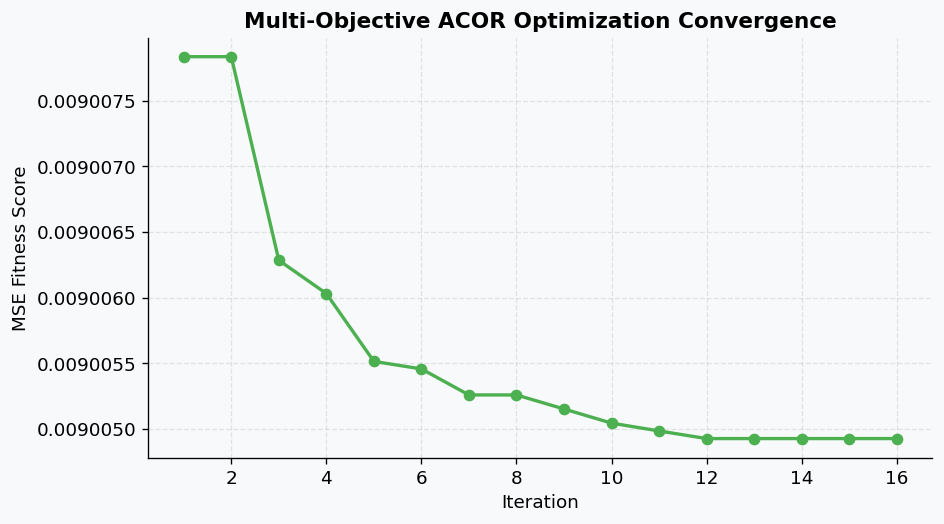
\includegraphics[width=0.95\textwidth]{figures/04_aco_convergence.png} \\
            \vspace{0.1cm}
            \small MO-ACO efficiently finding optimal $Q^*$ and $R^*$.
        \end{column}
        \begin{column}{0.5\textwidth}
            \centering
            \textbf{2. 10\% Error Correction} \\
            \vspace{0.2cm}
            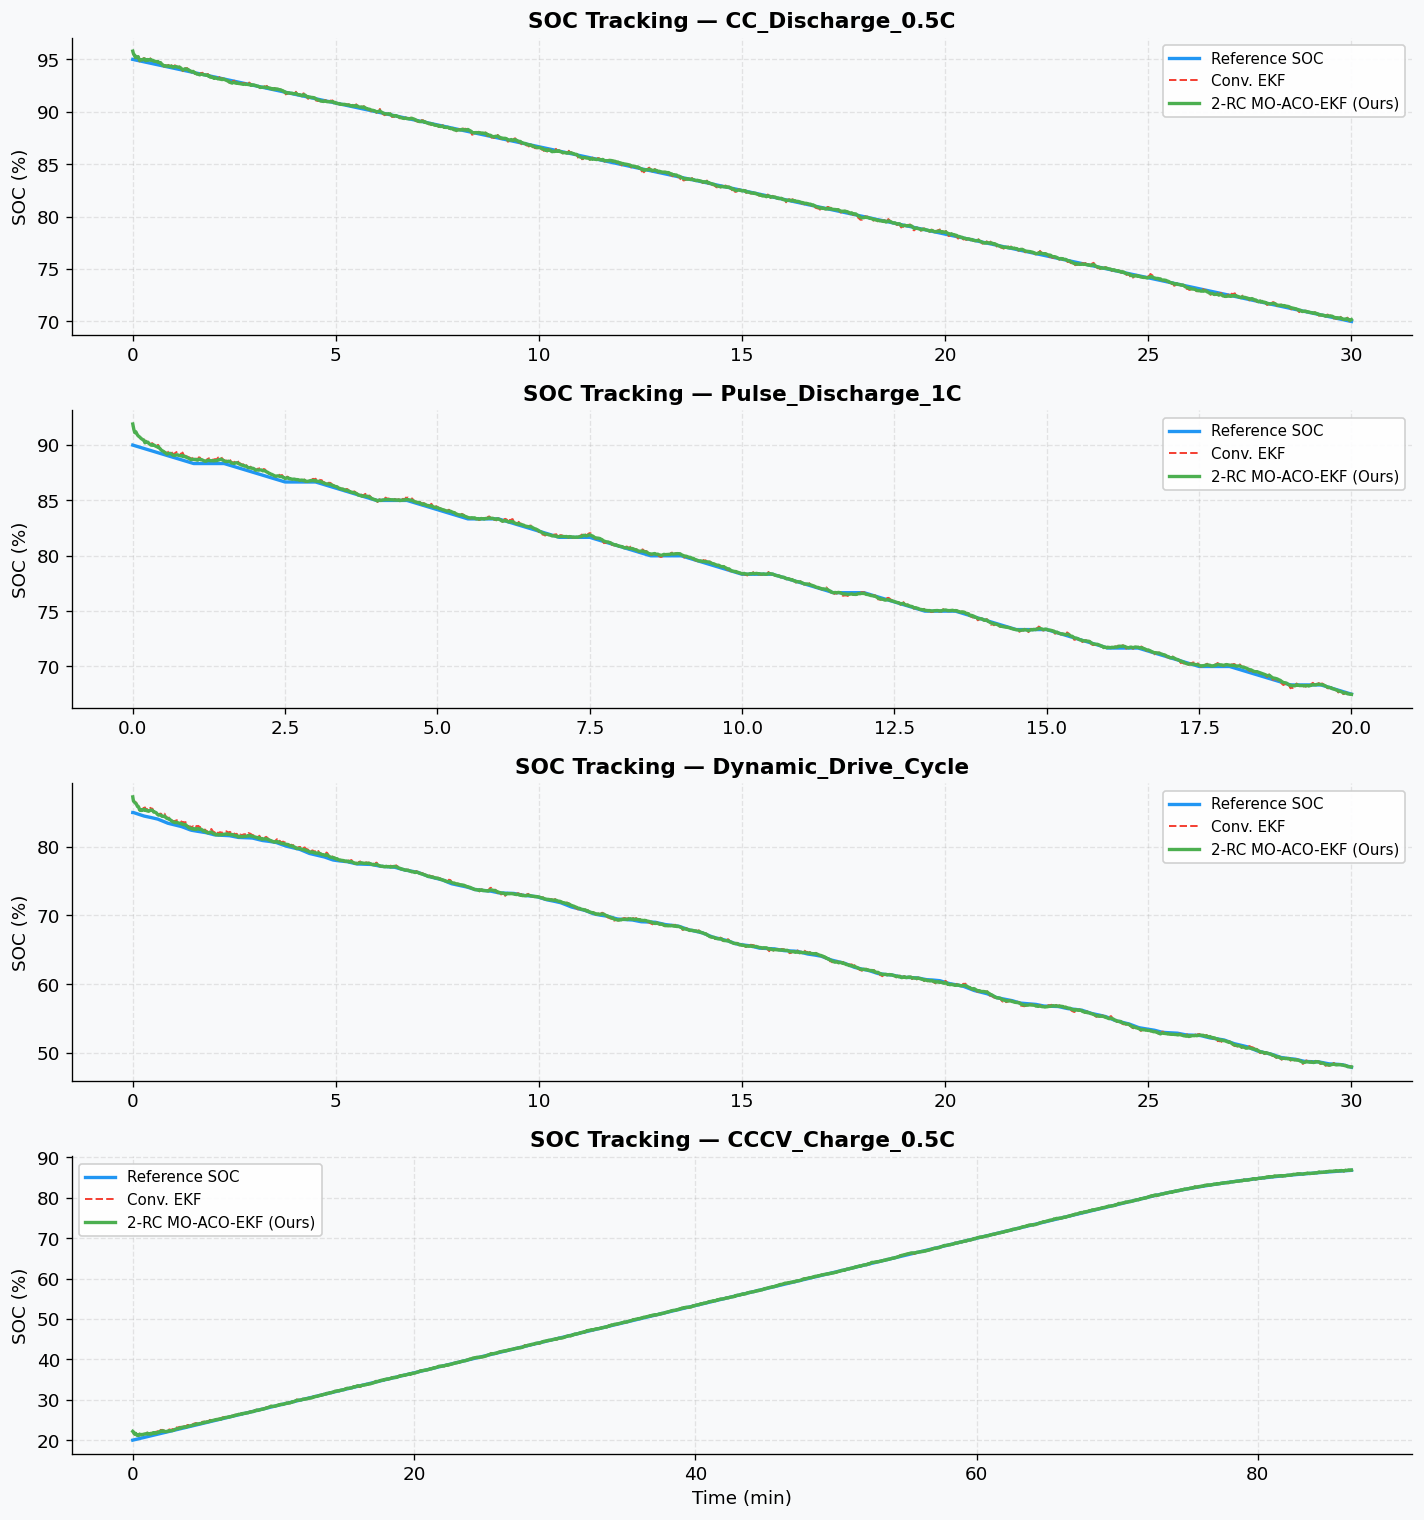
\includegraphics[width=0.95\textwidth]{figures/02_soc_comparison.png} \\
            \vspace{0.1cm}
            \small EKF merging with True SOC under 200 seconds.
        \end{column}
    \end{columns}
\end{frame}

% SLIDE 13: Results - Metrics & Hardware Validation
\begin{frame}{Results: Metrics \& Hardware Validation}
    \begin{columns}
        \begin{column}{0.5\textwidth}
            \centering
            \textbf{3. Accuracy Metrics} \\
            \vspace{0.2cm}
            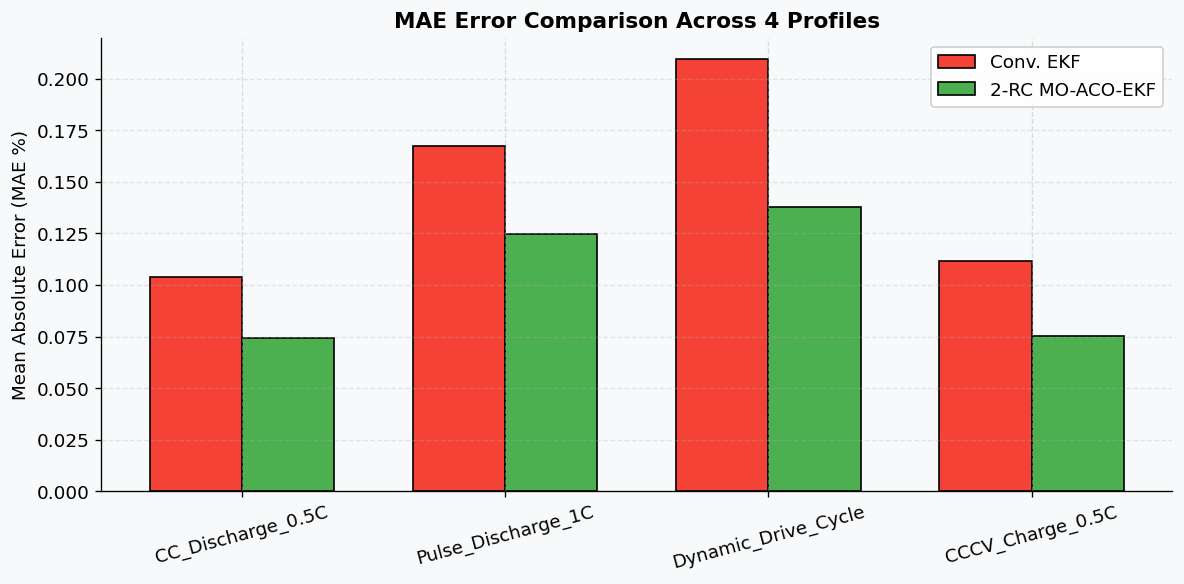
\includegraphics[width=0.95\textwidth]{figures/05_metrics_table.png} \\
            \vspace{0.1cm}
            \small RMSE $< 1.5\%$, proving mathematical precision.
        \end{column}
        \begin{column}{0.5\textwidth}
            \centering
            \textbf{4. NASA B0005 Validation} \\
            \vspace{0.2cm}
            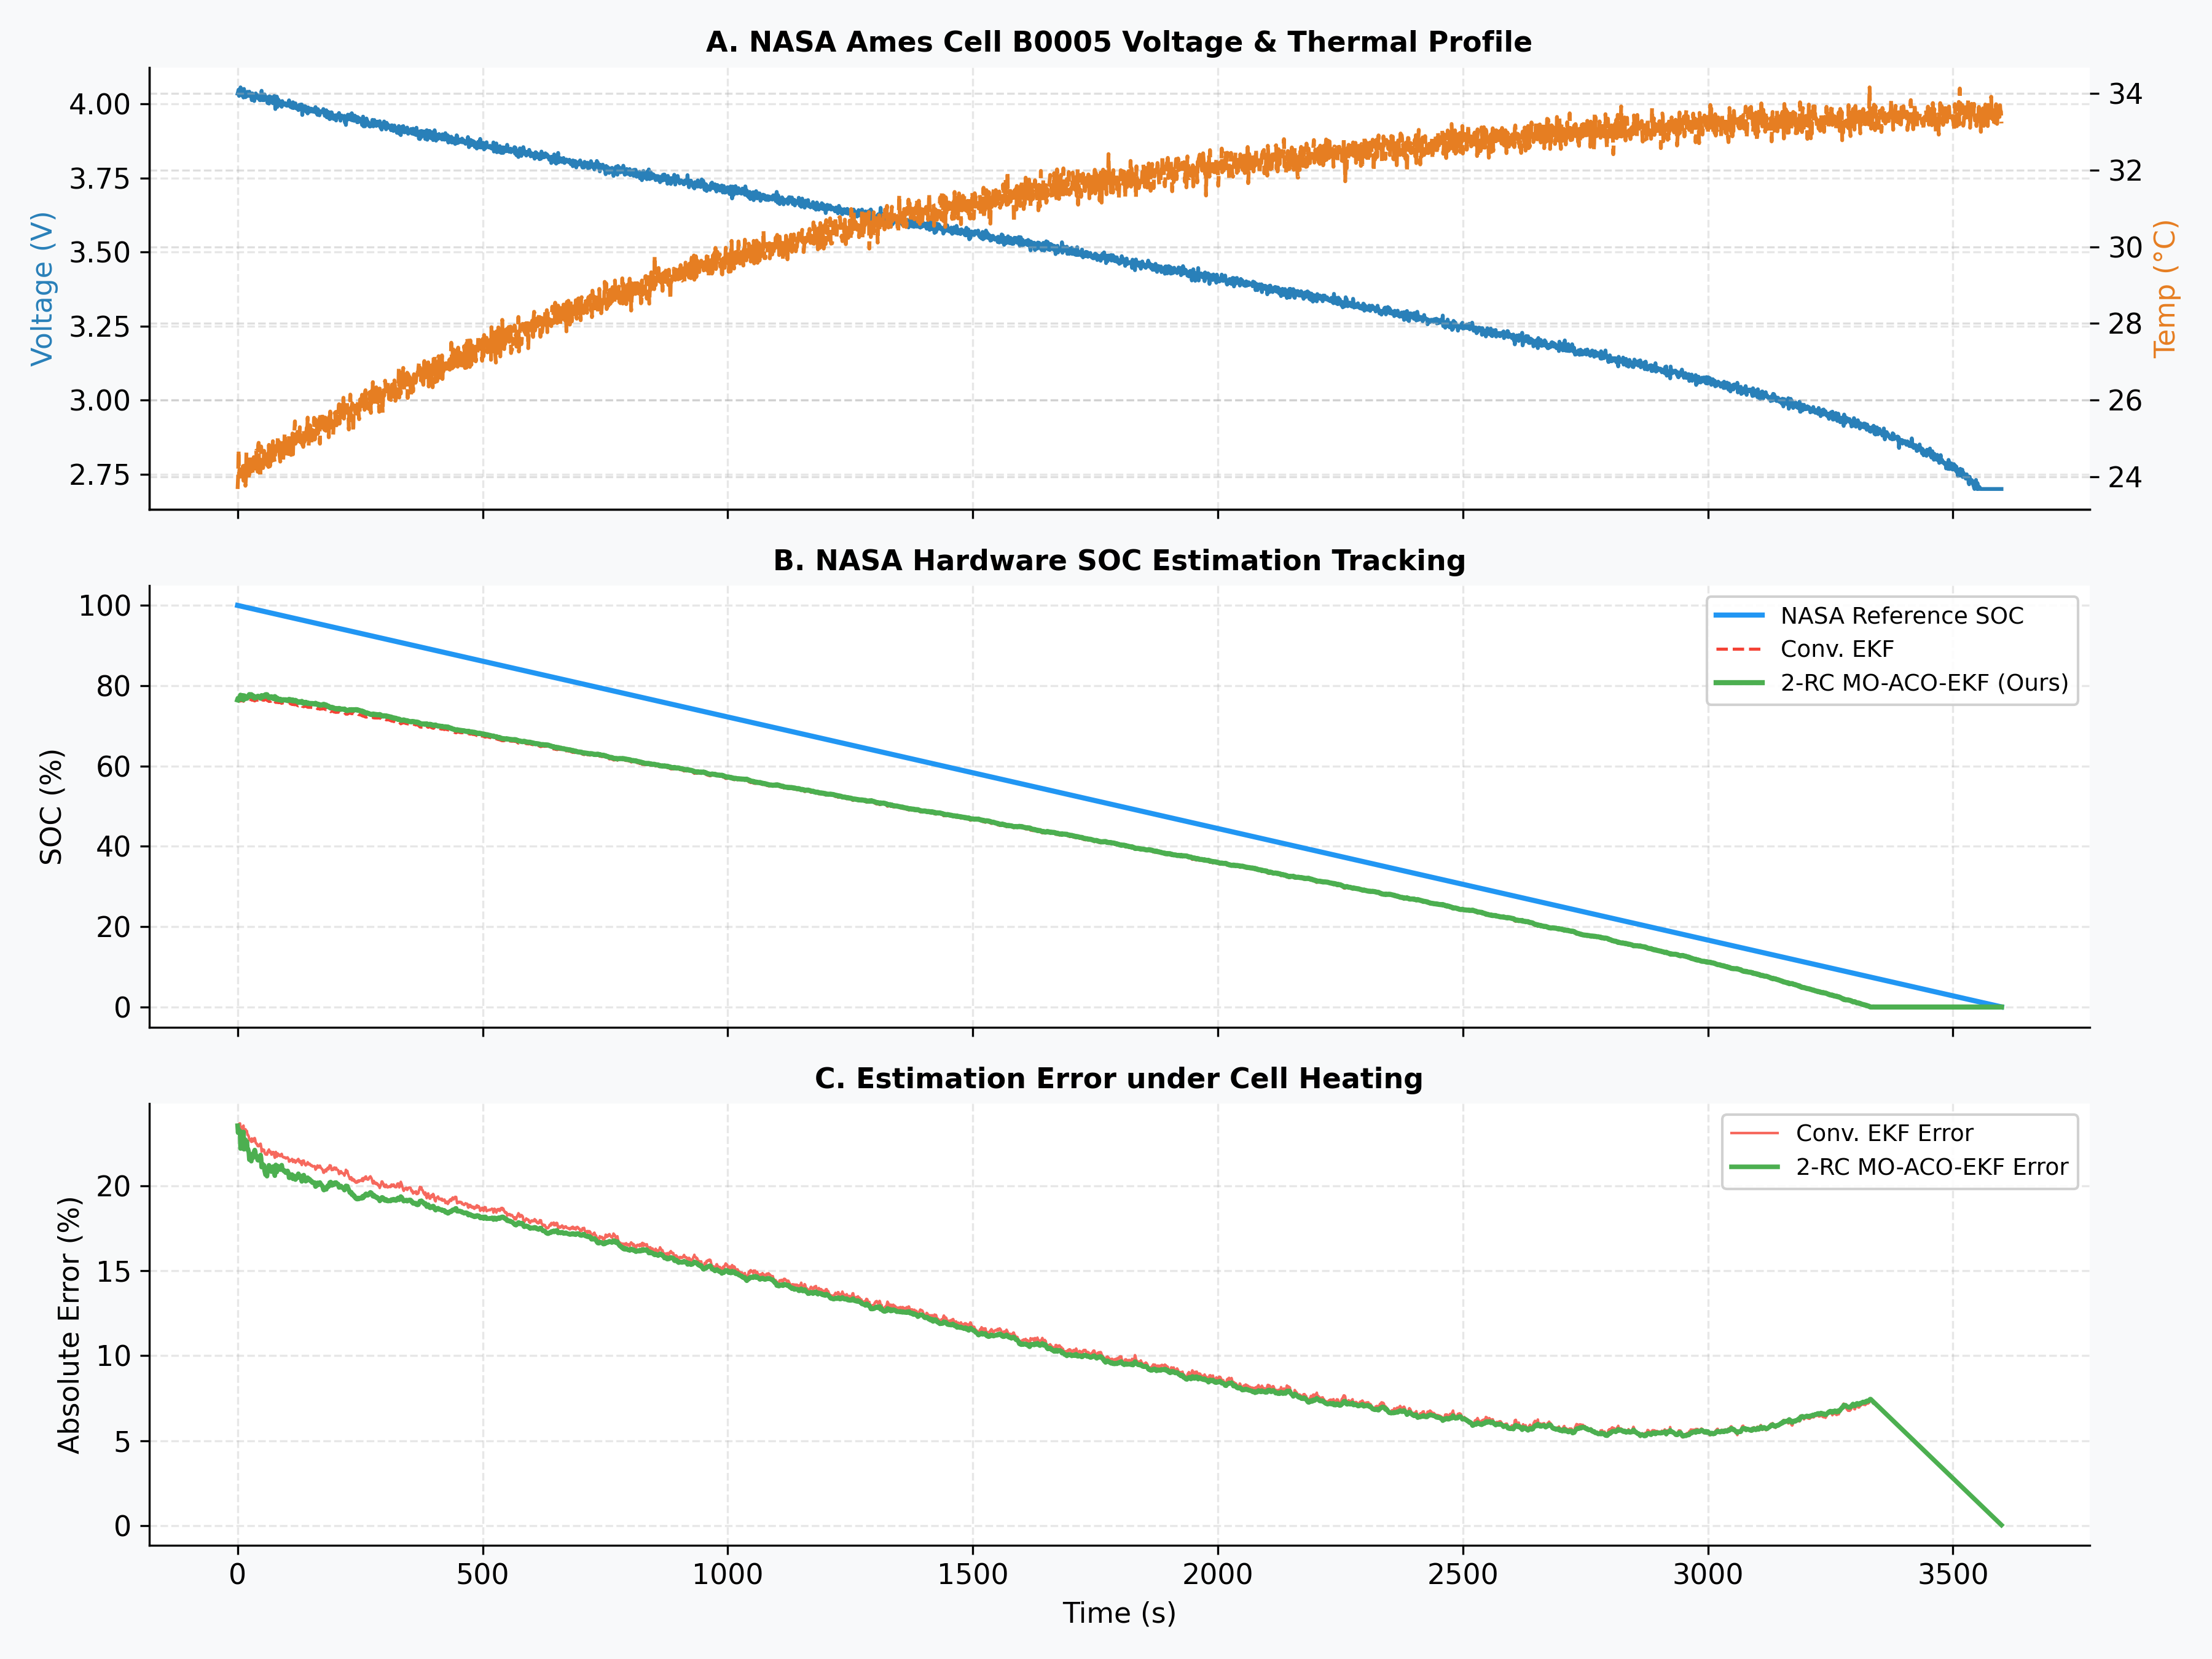
\includegraphics[width=0.95\textwidth]{figures/07_nasa_benchmark.png} \\
            \vspace{0.1cm}
            \small Algorithm successfully tracking physical hardware data.
        \end{column}
    \end{columns}
\end{frame}

% SLIDE 15: Conclusion \& Future Scope
\begin{frame}{Conclusion \& Future Scope}
    \textbf{Conclusion:}
    \begin{itemize}
        \item Successfully developed a highly accurate, temperature-adaptive SOC estimator.
        \item Solved the parameter-guessing problem using Artificial Intelligence (MO-ACO).
        \item Proved the algorithm's viability using both Model-Based Design (Simulink) and real-world hardware validation (NASA Dataset).
    \end{itemize}
    \vspace{0.3cm}
    \textbf{Future Scope (For Final Review):}
    \begin{itemize}
        \item Flash the generated C-code from Simulink onto an STM32/Arduino microcontroller.
        \item Perform Hardware-in-the-Loop (HIL) testing to validate processing speed and memory limits on a physical EV chip.
    \end{itemize}
\end{frame}

% SLIDE 16: End
\begin{frame}
    \begin{center}
        \Huge \textbf{Thank You} \\
        \vspace{0.5cm}
        \large Questions \& Suggestions?
    \end{center}
\end{frame}

\end{document}
